% !TEX root = ../main.tex
\section{Approach}
\label{sec:approach}
This section describes a method for estimating poses of noisy square fiducial tags using RGBD data. Unlike previous methods, the detected corners of the tag are treated as approximated locations of the true corners. Using the corners, the method implicitly evaluate the depth data and RGB data as two independent observations and fuse them in a meaningful way.

There are three distinct components to this method. First, we find the plane in $SO(3)$ containing the tag using depth data. Secondly, an approximate pose is computed using the depth plane and the corners from tag detection. Finally, the method refines the initial pose using the RGB data. Each component is described in detail in the following subsections and illustrated in Fig. 

\subsection{Depth Plane Fitting}
With a calibrated RGBD sensor, depth and RGB streams are registered to the same frame. The square patch of points in the depth image defined by the $g$ also contains the range information of the tag. Here we take advantage of the planar characteristic of the tag. By fitting a plane over the range data, we can constrain the pose of the tag to be on the plane.

The raw range data retrieved from the Kinect One sensor are usually noisy as illustrated by Figure \ref{fig:depth_data}. Specifically, borders of the tag and some of the dark regions of the tag produce highly unreliable range data. Therefore, we first filter the data by removing points too far from the median before fitting the plane. Nevertheless, the remaining points could have a large variance depending on the lighting condition and the magnitude of the plane rotation. The accuracy of the plane and tag pose is directly affected by the noise level of data. In fact, we want to characterize the uncertainty and weight the initial estimation accordingly during the fusing stage.

In implementation, we used a Bayesian plane fitting algorithm described in [Uncertainty Analysis] which computes the Hessian Normal parameters of a plane through optimizing
\begin{IEEEeqnarray}{c}
\min _{\boldsymbol{\hat{n}}, d} \sum_{j=1}^{N} 
	\frac{(p_j(\boldsymbol{\hat{n}} \cdot \boldsymbol{\hat{m}_j}) -d)^2}
		 {(\boldsymbol{\hat{n}} \cdot \boldsymbol{\hat{m}_j})^2\sigma ^2\{\bar{p}_j \} }
\label{eq:gaussian_noise}
\end{IEEEeqnarray}
The algorithm in the paper assumes a radial Gaussian noise in the range data $p_j$ with the standard deviation modeled by a function in the form
\begin{IEEEeqnarray}{c}
\sigma \{ \bar{p_j} \} = \frac{kd^2}{ \| \boldsymbol{\hat{n}} \cdot \boldsymbol{\hat{m}_j} \| } 
\IEEEeqnarraynumspace
\label{eq:gaussian_noise}
\end{IEEEeqnarray}
where $\boldsymbol{\hat{n}}$ is the local normal to the planar surface of the depth point and $\boldsymbol{\hat{m_j}}$ is the measurement direction for the sensor for point $p_j$. The coefficient $k > 0$ is an estimated value obtained from sensor calibration. In our implementation, we obtained $k$ by simplified the results from [Kinect Noise Model paper]. 

Another important result we used from [] is the covariance matrix for the plane-parameters. The covariance matrix is obtained by taking the \textit{Moore-Penrose generalized inverse} of Hessian matrix computed from the Lagrangian. The covariance characterizes the uncertainty of the plane and defines the refinement regions of the pose later in the pipeline. 

\begin{figure}
\centering
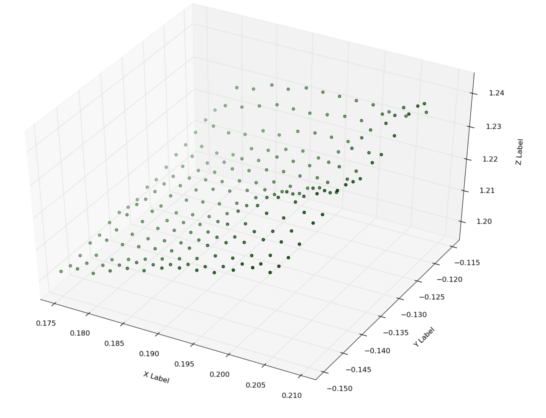
\includegraphics[width=\columnwidth]{figs/depth_plane_fig}
\caption{The depth points of the Apriltag plane. The points are noisy but good for an approximate estimation.}
\label{fig:depth_data}
\end{figure}

\subsection{Initial Pose Estimation}
The pose of the tag can be described as the transformation from tag's frame to the sensory frame of the robot given by $[R, \boldsymbol{t}]$. However, the depth plane $D [ \boldsymbol{\hat{n}}, d]$ alone is insufficient to determine the transformation because it only defines 3 DOF in a 6 DOF space. Furthermore, the center of the tag must align with the center of the plane and thus further constrain 2 DOF. However, there are still infinite number of valid poses rotating about the normal $\boldsymbol{\hat{n}}$. One solution is to constrain the pose by using a corner as an extra point correspondence to solve for the optimal rotation. However, the accuracy of this method largely depends on the depth accuracy of the chosen corner point. 

An alternative is to use all 4 detected corners as 4 pairs of point correspondences for the optimization. We projected the detected corners onto $D [ \boldsymbol{\hat{n}}, d]$ to get the coordinates $p = [p_1, p_2, p_3, p_4]$ in the robot sensory frame. The corner coordinates $q = [q_1, q_2, q_3, q_4]$ in the tag frame can be easily calculated since the tag is a square plane. We define the center of the tag as the origin, the corner coordinates are simply the location of the corners on a Cartesian plane. Given two sets of 3D point correspondences, this can be computed as a rigid body transformation estimation [Reference to SVD 3D rigid body]. Solving for the optimal transformation $[R, \boldsymbol{t}]$ requires minimizing a least squares error objective function given by:
\begin{IEEEeqnarray}{c}
[R, \boldsymbol{t}] = \argmin _{R \in SO(3), \boldsymbol{t}\in \mathbb{R}^3} \sum_{i=1}^{n} w_i \| R \boldsymbol{p_i} + \boldsymbol{t} - \boldsymbol{q_i}\| ^2
\IEEEeqnarraynumspace
\label{eq:rigid_body}
\end{IEEEeqnarray}
There are numerous approaches to solve Eq. \ref{eq:rigid_body}. Since we have very few correspondences and they are assumed to be correct, it can be computed quickly using SVD:
\begin{IEEEeqnarray}{rCl}
& \bar{p} = \frac{1}{N} \sum_{i=1}^{N} p_i \qquad p_{ci} = p_i - \bar{p} \\
& \bar{q} = \frac{1}{N} \sum_{i=1}^{N} q_i \qquad q_{ci} = q_i - \bar{q} 
\end{IEEEeqnarray}
\begin{IEEEeqnarray}{rCl}
p_{c}^{\top}q_c &= U\Sigma V^\top \\
R & = VU^\top\\
\boldsymbol{t} & = \bar{q} - R\bar{p}
\end{IEEEeqnarray}
$R$ and $t$ are the corresponding rotation and translation components of the the transformation. The above approach minimizes the least square error of the transformation and it is robust to small errors in the correspondences. The resulting pose obtained from the range data, although not accurate, is robust to noise and provide a good approximation for the true pose. 

\subsection{Pose Refinement}
\begin{figure}
\centering
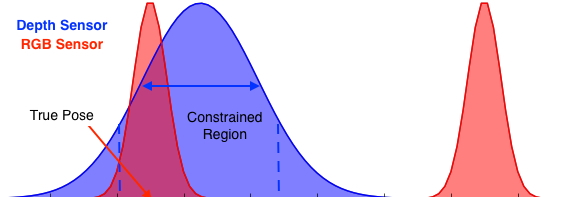
\includegraphics[width=\columnwidth]{figs/optimization_visualization_fig}
\caption{An abstract visualization of the optimization constraints. The blue curve is the initial pose estimation obtained from the depth plane. The red curves are the ambiguous poses from the RGB image. We constrained the region of optimization based on how well we fit the depth plane.}
\label{fig:calib}
\end{figure}
Given the initial pose estimate of the tag and the RGB image, we can refine the pose that minimizes the reprojection error. Given camera model $K$, initial rotation and translation estimates $R_{init}$ and $t_{init}$
\begin{align*}
\hat{y} &= K[(R_{init} + \Delta R)x + (t_{init} + \Delta t)]\\
&\underset{\Delta R, \Delta t}{\mathrm{min}} (y - \hat{y})\\
&\text{subject to:} \\
& |\Delta R| <= \Gamma_R, \; |\Delta t| <= \Gamma_t\\
\end{align*}
The challenge here is to determine the region $\Gamma_R$ and $\Gamma_t$ which the initial pose estimate can be adjusted. If we unbound $\Delta R$ and $\Delta t$ intheon Apriltag detection algorithmson Apriltag detection algorithm the optimization, the solution might converge to a pose optimal for the reprojection error but far away from the true pose due to perceptual ambiguity. On the other hand, if we constrain the optimization too much, the final pose might not be far away from the true pose because of the inaccurate initial estimation. We recognize that the bound of on this optimization is related to the variance of the initial pose estimation. In one extreme, if there is no uncertainty in the depth camera and the range data are perfect, we don't need to further refine the pose of the tag. Similarly, if we don't have any depth information (uncertainty of the initial estimate is infinity), then the best we can do is find the pose solely based on the reprojection error which is the same as solving the unbounded optimization problem. Thererfore, this becomes a constrained optimization problem where the bound on the independent variables of $\Delta R$ and $\Delta t$ is proportional to the covariance of our estimated depth plane parameters. In our implementation, we used the trust-region algorithm to bound the optimization. The scaling threshold parameter is emperically tested to yield the best results for our robot. 

The key insight to our method is that it harness the different strength of RGB and depth information during the pose optimization process. By considering all the points on the tag, the depth data is more robust to noises in the scene. However, range data is inherently inconsistent and the pose is thus imprecise. In contrast, the advantage of RGB image is that the corners can be detected at a sub-pixel precision. It is useful for refinement optimization.  